\documentclass[a4paper]{article}
\usepackage{hyperref} 
\usepackage[T1]{fontenc}
\usepackage[utf8]{inputenc}
\usepackage{amsmath,amsfonts,amssymb}
\usepackage[margin=1in]{geometry}
\usepackage[french]{babel}
\usepackage{graphicx}
\usepackage{subcaption}
\usepackage{amsthm}
\newtheorem*{remark}{Remarque}

\title{\Huge{\textbf{PROJET S6 }: Amazones}\\
\rule{\linewidth}{0.1mm}}

\date{}

\begin{document}

\maketitle

\begin{center}
  \Large{Département Informatique\\
  S6-Année 2022-2023}
\end{center}

\begin{center}

\end{center}
\newpage
\tableofcontents
\listoffigures
\newpage


\section{Introduction}

Ce projet constitue une implémentation du jeu des amazones en appliquant diverses techniques de programmation et de conception tel qu'une séparation des joueurs et du serveur de jeu.

\subsection{Le jeu des amazones}
Le jeu des amazones est un jeu de plateau proche des échecs qui prend place sur un plateau de taille \emph{m * m} et qui oppose deux joueurs. A chaque tour ils doivent déplacer l'une de ses reines (qui se déplacent d'autant de cases que souhaité tant que c'est possible dans l'une des huit directions, comme aux échecs), puis lui faire tirer une flèche. Les flèches possèdent le même panel de mouvement que les reines, à l'exception faite qu'une fois placées elles ne peuvent pas être déplacée et condamnent donc les cases sur lesquelles elles se trouvent. Un joueur perd lorsqu'il ne peut plus déplacer ses reines.


\section{Le monde}
Le jeu des amazones prend place sur un plateau de taille et de forme variables. Cependant, la forme globale du plateau reste carrée. Toutes les cases sont elles aussi aussi carrées et numérotées de 0 à \emph{n-1} de gauche à droite et de haut en bas. Dès lors, il semble judicieux de représenter le monde sous forme d'un graphe non orienté. Chaque case du plateau correspond à un sommet et le passage d'une case à l'une de ses voisines est représenté par une arête. Chaque sommet a alors au plus huit arêtes. Cependant, un graphe est une structure de donnée abstraite et il faut donc parvenir à l'implémenter en C. Pour cela a été imposé la librairie \emph{GNU Scientific Library}, abrégée en GSL.

\subsection{Graphes et matrices d'adjacence}

Un graphe peut être représenté sous la forme d'une matrice d'adjacence. Soit un graphe de \emph{n} sommets, la matrice d'adjacence correspondante sera de taille $n * n$. Chaque ligne correspond à un sommet. Une arête allant du sommet \emph{i} au sommet \emph{j} est représentée dans la matrice par un nombre à la position\emph{(ij)}. Ce nombre correspondant à une direction est défini dans un \emph{enum}. Si l'arête menant le sommet \emph{i} au sommet \emph{j} n'existe pas, elle est symbolisée pas un zéro dans le graphe aux coordonnées \emph{(ij)}. La figure \ref{fig:rose} montre la liste des directions et les nombres associés :

\begin{figure}[h!]
    \centering
    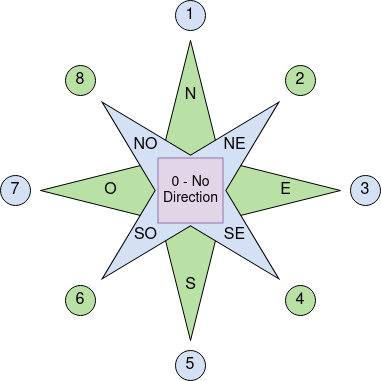
\includegraphics[width=0.4\textwidth]{Rose.png}
    \caption{Rose des vents et chiffres associés aux directions}
    \label{fig:rose}
\end{figure}

Par exemple, la figure \ref{fig:exemplematrice} montre la représentation abstraite d'un plateau $3 * 3$ sous forme de graphe, puis sous la forme d'une matrice d'adjacence. Plusieurs remarques ont leur importance : la première est que la matrice semble au premier abord symétrique mais ce n'est pas le cas. En effet, si l'élément de la matrice à la position \emph{(ij)} est non nul, il en va de même pour l'élément à la position \emph{(ji)}. Cependant, ces valeurs ne sont pas égales car pour passer du sommet \emph{i} au sommet \emph{j} il faut emprunter une direction particulière et pour passer du sommet \emph{j} eu sommet \emph{i} il faudra emprunter la position opposée (par exemple Sud et Nord). Ainsi, l'entièreté de la matrice doit être gardée. Il est tout de même possible de ne garder que le triangle supérieur ou inférieur car chaque direction n'en a qu'une opposée mais cela n'est pas rentable au niveau de la complexité des calculs et du code comparé au gain d'espace. Une deuxième remarque est que la matrice est particulièrement creuse car chaque sommet a au plus huit arêtes. La matrice devient d'autant plus creuse que le nombre de sommet augmente. Il est intéressant de trouver un moyen permettant de ne stocker que les informations utiles de la matrice. 


\begin{figure}[h!] 
    \centering
    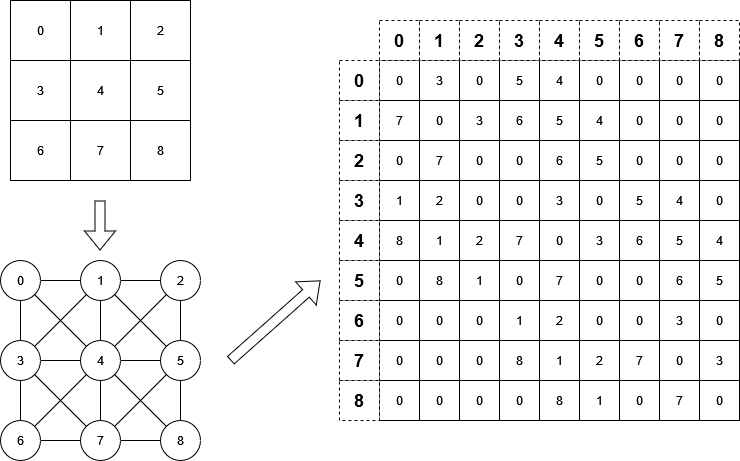
\includegraphics[width=0.8\textwidth]{matriceAdja.png}
    \caption{Exemple de matrice d'adjacence pour un plateau $3 * 3$.}
    \label{fig:exemplematrice}
\end{figure}


\subsection{GNU Scientific Library et Matrices CSR}

La GSL permet de représenter efficacement des matrices. Par "efficacement" est entendu "de manière optimisée". En effet la GSL propose différents types de représentation. Notamment ici est utilisé le format \emph{Compressed Sparse Row}, abrégé en CSR.

Le format CSR permet de stocker une matrice creuse sous la forme de trois tableaux nommés \emph{data}, \emph{col} et \emph{row\_ptr}. Les deux premiers tableaux ont une taille égale au nombre d'éléments non nul dans la matrice d'adjacence et le dernier tableau a pour taille le nombre de sommets plus un. Le tableau \emph{data} contient les éléments non nuls de la matrice dans leur ordre d'apparition (lors d'une lecture de gauche et droite et de haut en bas). Le second tableau indique la colonne sur laquelle se trouve les éléments non nuls. Par exemple, l'élément \emph{data[i]} se trouve sur la colonne \emph{col[i]}. Enfin le dernier tableau indique le nombre d'éléments sur les lignes. Par exemple, si $row\_ptr[1] = 2$ alors cela indique qu'il y a 2 éléments sur la première ligne (la ligne indicée 0). Si $row\_ptr[3] = 8$ alors il y a 8 éléments sur les 3 premières lignes (les lignes indicées de 0 à 2). Ainsi, $(row\_ptr[i] - row\_ptr[i-1])$ correspond au nombre d'éléments sur la $i^{ieme}$ ligne (la ligne indicée $i-1$).  Enfin, pour accéder aux éléments sur la $i^{ieme}$ ligne, les éléments du tableau \emph{data} situés entre $(row\_ptr[i-1])$ et $(row\_ptr[i])$ sont parcourus.

La figure \ref{fig:csr} représente les trois premières lignes de la matrice d'adjacence de la figure \ref{fig:exemplematrice}.

\begin{figure}
    \centering
    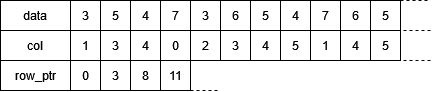
\includegraphics[width=0.8\textwidth]{csr.png}
    \caption{Exemple de matrice CSR.}
    \label{fig:csr}
\end{figure}

La GSL permet donc de représenter des matrices d'adjacence (creuses) en optimisant l'espace. Les matrices CSR sont utilisées tout au long du projet pour modéliser le plateau. Cependant, elles sont un type de matrices compressées particulières qui ne peuvent pas être modifiées avec les fonctions régulières de la GSL telle que \emph{spmatrix\_set}. Il est possible de décompresser une matrice CSR, modifier son contenu et de la recompresser. Or cette méthode est très coûteuse et a donc été évité, au profit d'une modification à la main des tableaux \emph{data}, \emph{col} et \emph{row\_ptr}.



\section{Affichage}

Dans l'objectif de pouvoir visualiser des parties et déboguer, une fonction d'affichage a été développée. Cette dernière permet d'afficher sur un terminal la plateau de jeu sous la forme d'un graphe. Chaque sommet correspond à une case du plateau de jeu et est symbolisé par un petit carré. Les reines sont représentés par les caractères unicode correspondants. De plus, la fonction affiche les arêtes reliant les sommets, ce qui permet de visualiser les déplacements possibles au sein du plateau. Lorsqu'une flèche est placée sur une case, les arêtes reliant cette dernière à ses cases voisines sont supprimées et les cases fléchées sont donc montrées comme des sommets sans arêtes. Enfin, de la couleur a été ajoutée lors du tour d'un joueur pour indiquer le mouvement effectué : la reine déplacée est verte, la case de laquelle elle provient est en rose et la positions de la flèche tirée est en cyan. La figure \ref{fig:affichage} expose l'affichage de l'état du jeu en milieu de partie.


\begin{figure}[h!]
    \centering
    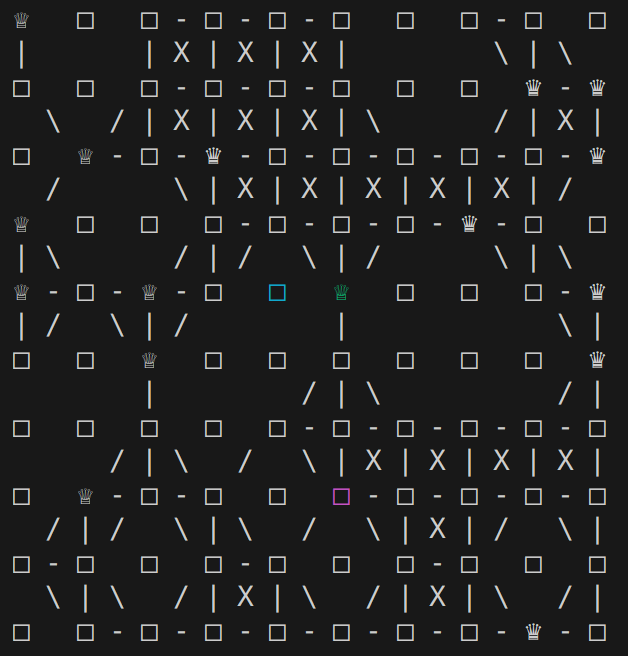
\includegraphics[width=0.6\textwidth]{affichage_amazons.png}
    \caption{Affichage sur terminal du jeu.}
    \label{fig:affichage}
\end{figure}

Cependant, il est important de mentionner que la fonction ne vérifie pas ni ne permet de vérifier que le graphe affiché est parfaitement formé. En effet, lors de l'affichage des arêtes, la fonction se contente de regarder si un sommets possède des arêtes au Sud-Ouest, au Sud, au Sud-Est et à l'Est, auquel cas elles sont affichées. La fonction admet donc que les sommets de l'autre côté de ces arêtes aient aussi une arêtes en sens inverse ramenant au sommet d'origine. Cette fonction est donc un ajout appréciable mais ne remplace pas des tests approfondis quant à la génération et à la modification des graphes.


\section{La dualité serveur-clients}

\subsection{Les clients}
Le client s'occupe d'une copie du plateau communiqué par le serveur puis met à jour son plateau de son côté selon ses propres coups et ceux adverses communiqués par le serveur. À chaque tour, le client soumet au serveur son coup selon sa stratégie.

Chaque client est partagé sous forme de bibliothèque dynamique et contient son implémentation des fonctions appelées par le serveur.


\subsection{Le serveur}
Le serveur se charge de fournir à chaque client une copie du plateau initialisé et de communiquer les coups de chaque joueur à l'autre joueur en vérifiant leur validité.

Le serveur charge les clients dynamiquement avec \emph{dlopen} et accède aux fonctions des clients avec \emph{dlsym}. Les étapes de la boucle de jeu se résument dans la figure \ref{fig:boucle}.

\begin{figure}
    \centering
    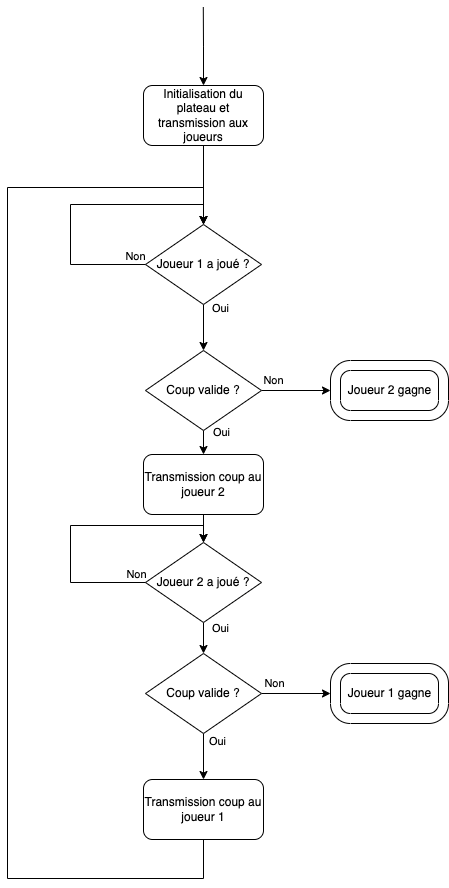
\includegraphics[width=0.6\textwidth]{bouclejeu.png}
    \caption{Boucle de jeu d'une partie d'amazones.}
    \label{fig:boucle}
\end{figure}

\subsection{Organisation du code}
Le projet est composé de plusieurs répertoires pour séparer l'implémentation du serveur et des clients. Cette séparation n'empêche pas le serveur et les clients d'utiliser les mêmes fichiers d'en-têtes, comme présenté dans le graphe des dépendances figure \ref{fig:dependance}. Une flèche d'un fichier A vers un fichier B indique que le fichier A dépend du fichier B. La partie purement serveur est entouré en bleu et celle purement client est entouré en rouge. Cette dernière permet la création de la bibliothèque dynamique \emph{player.so}, ce lien étant indiqué d'une flèche en gras. Aucun fichier ne dépend du fichier \emph{player.c} et son remplacement permet la création de différents joueurs et donc de plusieurs bibliothèques.


\begin{figure}
    \centering
    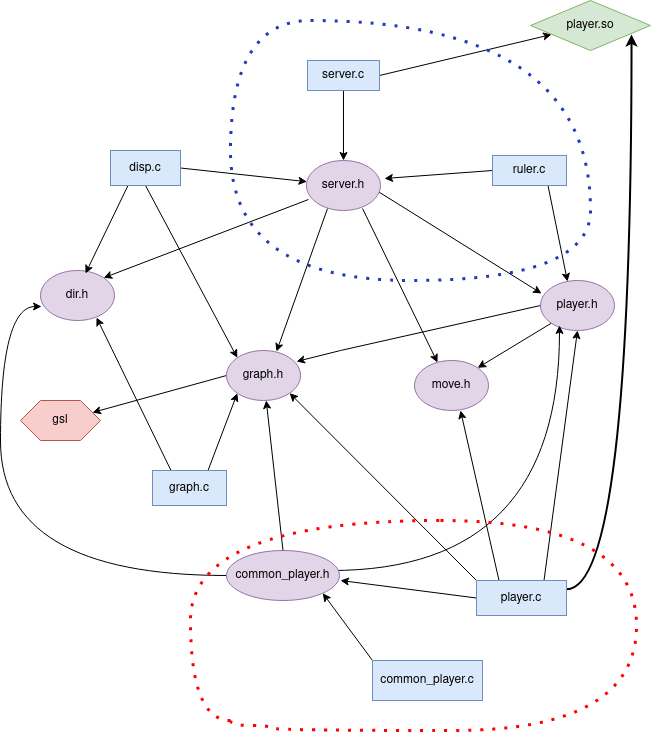
\includegraphics[width=0.7\textwidth]{dep c.png}
    \caption{Graphe des dépendances du code.}
    \label{fig:dependance}
\end{figure}


\section{Les stratégies}
Ce jeu rentre dans le cadre des jeux à somme nulle car les gains de l'un sont très exactement les pertes de l'autre. Certes, il est possible de faire des joueurs aléatoires mais, il existe plusieurs algorithmes dans le domaine de la théorie des jeux qui permettent de créer des joueurs un peu plus intelligents comme Minmax (avec et sans élagage alpha-bêta) ou Monte-Carlo.
\subsection{La stratégie aléatoire}
Une des stratégies les plus simples consiste à choisir aléatoirement une reine pouvant se déplacer, choisir aléatoirement une destination possible pour la reine, puis choisir aléatoirement une cible possible pour la flèche.
Cette stratégie est simple à implémenter et présente l'avantage de la rapidité de décision.
Cependant, une stratégie un peu plus intelligente suffit à battre cette stratégie aléatoire la plupart du temps.

\subsection{L'algorithme Minmax avec élagage alpha-bêta}
\subsubsection{Principe}
L'algorithme minmax consiste à construire un arbre (dit de recherche) des mouvements possibles et à effectuer une exploration complète de cet arbre jusqu'à un niveau donné tout en attribuant à chaque nœud un score selon l'heuristique choisie. C'est ainsi qu'il trouve le meilleur mouvement après une imagination du déroulement de la partie.

L'élagage alpha-bêta est utilisé pour améliorer la complexité de minmax. Celui-ci permet de couper des branches de l'arbre de recherche s'il est sûr qu'il n'y aurait pas de mouvement meilleur que celui déjà choisi.


\subsubsection{Heuristiques}
Dans le cadre d'une application il est nécessaire de tester des heuristiques pour en déterminer certaines qui soient performantes face au problème à résoudre. Pour le jeu des amazones, il est possible de s'intéresser à plusieurs paramètres pouvant affecter le score de chaque coup rendu par l'heuristique. Notamment peuvent être retenus le territoire, le nombres de coups disponibles, le nombres de pièces pouvant encore bouger, la capacité d'un coup à éliminer du jeu une pièce adverse en réduisant à néant ses possibilités de déplacement, etc. Par exemple, une première heuristique employée était de comptabiliser les coup possibles du joueur en attribuant des points en fonction de la distance parcourue par les reines. Plus un coup parcourt de distance plus il est compté comme important. La sommes des points correspond au score du premier joueur. A cette valeur est soustrait le même score mais calculer pour l'adversaire :
\begin{equation}
    score_{tot} = score_{joueur} - score_{adversaire}
\end{equation}
Cette heuristique propose un compromis entre étendre sa maîtrise du territoire et diminuer les possibilités de mouvement de l'adversaire. De plus, elle peut être modifié de sorte à pondérer le score des deux joueurs : 
\begin{equation}
    score_{tot} = k * score_{joueur} - score_{adversaire}
\end{equation}
où k est une constante.

Cela permet de faire plus ou moins valoriser la défense ou l'attaque. En effet, pour $k < 1$ le score du joueur actuel est moins pris en compte et donc l'objectif est plutôt de diminuer les possibilités de déplacements de l'adversaire. A l'inverse, en prenant $k > 1$ la défense est préférée face à l'attaque. Cependant, lors de l'observation de nombreuses partie, il a été remarqué que le joueur qui commence a de plus grande chance de gagner car il a la main sur l'attaque et donc la gestion du terrain. Si le joueur joue en premier, il est donc intéressant de prendre $k < 1$ pour jouer de manière agressive. Et inversement, si le joueur joue en second, il est préférable de favoriser la défense et de prendre $k > 1$. Enfin il est aussi possible d'alterner entre différentes valeurs de k au fur et à mesure de la partie en fonction de l'avancement de celle-ci et des positions des deux joueurs.

Une autre variante consiste à valoriser l'entrave des reines ennemies en gardant le plus de directions possibles pour les reines du joueurs lors des prochains tours :
\begin{equation}
    score_{tot} = score_{joueur} - score_{adversaire} 
    + k_2 * (dir\_restantes_{joueur} - dir\_restantes_{adversaire})
\end{equation}
où $k_2$ est une constante.


D'autres heuristiques ont aussi été testées en gardant le même principe que celle de base, c'est à dire compter le nombre de case possible pour chaque reine avec la valeur de chaque cas correspondant à la distance entre celle-ci et la reine. Les scores de chaque reine sont calculés indépendamment les uns des autres puis sont multipliés par un facteur x. Le calcul de x est le suivant : $x = 1.k$ où $k$ est le nombre de directions possibles pour la reine. Par exemple pour 3 directions empruntables, $x = 1.3$. Comme les deux autres heuristiques on calcule le score totale de la façon suivante :

\begin{equation}
    score_{tot} = (1 + \frac{rba - rbj}{rt})* score_{joueur} - (1 + \frac{rbj - rba}{rt})* score_{adversaire}
\end{equation}

Avec :
\begin{itemize}
    \item rbj : le nombre de reines bloquées pour le joueur.
    \item rba : le nombre de reines bloquées pour l'adversaire.
    \item rt : le nombre total de reines par joueur.
\end{itemize}
Ce facteur rajouté en plus permet si des coups ont des scores proches, de favoriser la prise des pièces de l'adversaire ou le sauvetage de nos pièces.

\subsection{Coût des stratégies}
Le calcul des mouvements possibles se fait de proche en proche selon chaque direction en vérifiant l'existence d'une arête de la direction considérée dans la matrice du plateau sous format CSR. De plus, l'algorithme minmax demande énormément de calculs des déplacements possibles. Cela a pour conséquence une complexité très importante et il a donc fallu réfléchir à différentes stratégies pour diminuer la dite complexité. En particulier, chaque calcul des mouvements possibles allouait et libérait un tableau et l'allocation unique des tableaux en début de partie pour tous les calculs a permis de réduire grandement le temps de calcul.


\section{Conclusion}

Pour conclure, le projet possède plusieurs fonctionnalités comme la création de différents plateaux de jeu mais aussi une interface client/serveur. Cette interface offre la possibilité de créer plusieurs joueurs avec des stratégies différentes pouvant s'affronter sur le serveur. Quant au serveur, il est là pour annoncer le gagnant et vérifier que personne ne fait de coup invalide.

Une piste d'amélioration de notre projet est d'essayer d'optimiser encore plus l'algorithme minmax afin d'augmenter la profondeur des calculs mais aussi d'avoir plus de temps pour peaufiner nos stratégies et heuristiques.

\end{document}
